\subsection{Solve a real problem}

The history of the internet is littered with solutions to non-problems.
It is very easy as scientists and engineers to get excited about what is possible, without considering if it is actually
useful. So it is important to consider if having access to your data is actually going to solve a real problem that your
users have. This is not the same thing as saying that their is a \emph{demand} for your data, because it is entirely possible 
the you can solve a problem that users don't currently realize they have.
Maybe your major task is to let he see how useful your data can be.\\

\subsubsection*{Suggested strategies} 

\begin{itemize}
    \item Put yourself in your user's shoes, and consider how your data may be of practical benefit.
    % \item Next we have to find a way to let him see because they are important to him and how he can benefit from using them in his daily life.
    % \item If the data is updated periodically, it is necessary to analyze what type of variations are important in the user's daily life.
    % Conduct a market study and see if there are already products that offer this information.
    % If this is the case, it will be analyzed because it is attractive to the user and try to improve it.
\end{itemize}

\subsubsection*{In the context of Aire Guru \ldots} 

Aire Guru allows users to see their exposure to air pollution without the need to carry an air monitoring device.
This has not previously been possible. 
Our post-launch survey results indicate that users found this not only interesting, but also strongly desirable, 
particularly given the health consequences that Aire Guru explains in the context of their exposure.\\

By providing geographically specific data, in both historical and current hourly timeframes, users are able
to control their exposure, which in some cases leads directly to the avoidance of serious negative health outcomes.\\

\begin{figure}[ht]
    \centering 
    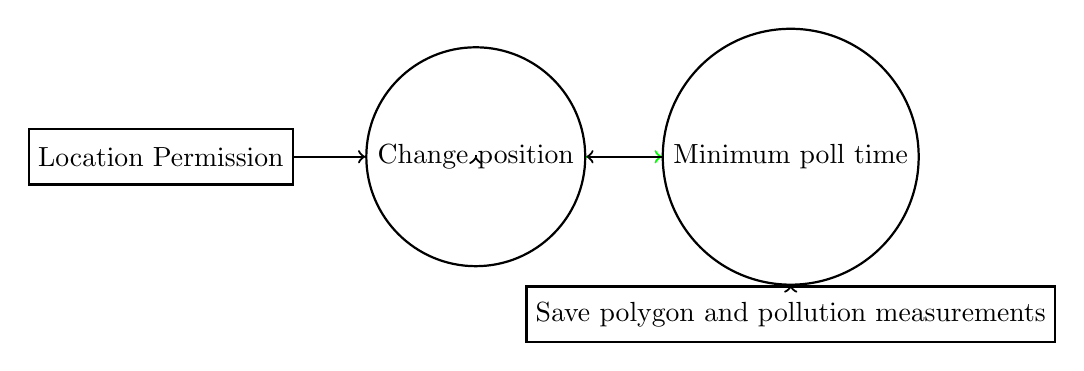
\begin{tikzpicture}[thick]
        \node[draw,rectangle,minimum size=20] (a) {Location Permission};
        \node[draw,circle,minimum size=6,right of= a, node distance=4cm] (b) {Change position};
        \node[draw,circle,minimum size=5,right of= b, node distance=4cm] (c) {Minimum poll time};
        \node[draw,rectangle,minimum size=20,below of=c, node distance=2cm] (d) {Save polygon and pollution measurements};
        \draw[->] (a) to (b);
        \draw[->] (b) to (b);
        \draw[->,green] (b) to (c);
        \draw[->] (c) to (d);
        \draw[->] (c) to (b);
    \end{tikzpicture}
    \caption{Collecting user location}
\end{figure}

\begin{figure}[ht]
    \centering
    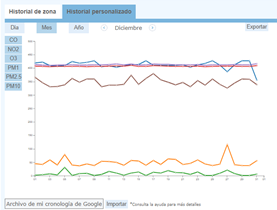
\includegraphics[width=8cm]{importedDataDecember}
    \caption{Personal Records. December}
\end{figure}